%%%%%%%%%%%%%%%%%%%%%%%%%%%%%%%%%%%%%%%%%%%%%%%%%%%%%%%%%%%%%%%%%%%%%%
% How to use writeLaTeX: 
%
% You edit the source code here on the left, and the preview on the
% right shows you the result within a few seconds.
%
% Bookmark this page and share the URL with your co-authors. They can
% edit at the same time!
%
% You can upload figures, bibliographies, custom classes and
% styles using the files menu.
%
%%%%%%%%%%%%%%%%%%%%%%%%%%%%%%%%%%%%%%%%%%%%%%%%%%%%%%%%%%%%%%%%%%%%%%

\documentclass[12pt]{article}

\usepackage{sbc-template}
\usepackage{underscore}
\usepackage{graphicx,url}

%\usepackage[brazil]{babel}   
\usepackage[utf8]{inputenc}  

     
\sloppy

\title{Tutorial de instalação das ferramentas GCC, GDB, Nasm, Objdump, Kdbg e outras ferramentas de edição de texto em uma máquina com o Sistema Operacional Windows 10 - Passo a Passo}

\author{José Inaldo dos Anjos Junior\inst{1}}


\address{Colegiado de Computação -- Universidade Estadual de Santa Cruz
  (UESC)\\
  Ilhéus -- BA -- Brazil
  \\Departamento de Ciências Exatas e Tecnológicas -- DCET
  \email{\{inaldoanjosjr\}@gmail.com}
}

\begin{document} 

\maketitle

\begin{abstract}
  The basic software is commissioned, among other things, by the communication between the hardware of the machines and the services of the highest level. Some typical examples of basic software are the BIOS of a personal computer, the kernel of operating systems such as UNIX or Windows NT, the builders themselves for machine languages, etc. In this way, perhaps the term basic software should be exchanged for essential software, given its importance in the nature of the products that this software concept covers.
\end{abstract}
     
\begin{resumo} 
  O software básico é incumbido, dentre outras coisas, pela comunicação entre o hardware das máquinas e os serviços de mais alto nível. Alguns exemplos típicos de softwares básico é o BIOS de um computador pessoal, o kernel de sistemas operacionais como o UNIX ou o Windows NT, os próprios montadores para linguagens de máquina, etc. Desta maneira, talvez o termo software básico devesse ser trocado por software essencial, dada sua importância na natureza dos produtos que este conceito de software abrange.
\end{resumo}


\section{Introdução}

O Assembly foi provavelmente a primeira linguagem de programação da história, surgida na década de 50, época em que os computadores ainda usavam válvulas. A idéia do Assembly é usar um comando em substituição a cada instrução de máquina. Ao invés de usar instruções como 10101011, no Assembly, podem ser usados outras instruções bem mais fáceis de entender e de memorizar, como add, div, mul, and, or, not, etc. Por exemplo, a instrução "add" faz com que o processador some duas variáveis; "add x, y" por exemplo, soma os valores de x e y.

Desta maneira, o compilador transforma o código escrito em Assembly em linguagem de máquina, que finalmente poderá ser entendida pelo processador. Por causa desta característica de permitir trabalhar diretamente com as instruções do processador, o Assembly é uma linguagem de baixo nível. Porém, não significa que ela seja inferior, mas apenas que ela manipula diretamente as instruções e endereços de memória e, por isso, é mais trabalhosa e voltada para o desenvolvimento de aplicações otimizadas.

Neste breve relatório, mostraremos um passo a passo de que maneira as ferramentas foram instaladas na máquina, afim de ficar apto para realizações de desenvolvimento para a programação de baixo nível.

\section{Instalação} \label{sec:firstpage}

Para realização deste tutorial foi usada uma máquina com Sistema Operacional (SO) Windows. Desta maneira, foi preciso realizar a instalação do SO Ubuntu, versão para desenvolvimento, disponível na loja Microsoft, como descrito a seguir.

\subsection{SO Ubuntu na máquina Windows 10}

Para instalar uma distribuição Linux no computador, é necessário ter um processador de 64 bits rodando na máquina e o Anniversary Update (Versão 1607) ou versão superior. Além disso, a versão do Ubuntu a ser instalada se trata de versões voltadas para desenvolvedores, ou seja, sem ambiente gráfico.

 \begin{enumerate}
   \item Procure pela distribuição Linux desejada na Microsoft Store: Ubuntu, OpenSUSE ou SLES. No caso atual, foi utilizado Ubuntu;
   \item Após encontrar sua distribuição, faça o download;
   \item Enquanto o sistema faz a instalação, clique na caixa da Cortana e pesquise por “Ativar ou desativar recursos do Windows";
   \item Na janela que será exibida, procure e marque a opção “Subsistema do Windows para Linux” e pressione OK;
   \item Aguarde até o fim da instalação. Será necessário reiniciar o seu computador antes de prosseguir. \textbf{Observação:} Lembre-se de conferir se o download da distribuição Linux já está concluído;
   \item Após reiniciar, vá até o menu Iniciar e abra a distribuição do Linux que você acabou de baixar;
   \item Seja qual for a distribuição baixada, após a inicialização será necessária que esta faça uma instalação. Após será solicitado para que crie um nome de usuário UNIX e uma senha;
   \item Pronto, ambiente de desenvolvimento pronto para ser utilizado.
 \end{enumerate}

\subsection{GCC}

O GCC é um pacote de compiladores que dentre outras linguagens de programação como C/C++ \cite{gatliff1999embedding}, o desenvolvedor consegue compilar um código fonte (source), gerando um binário para o sistema operacional utilizado, aqui no nosso caso o Ubuntu. Além de compilar o código fonte, o GCC também possui um depurador (debugger) que ajuda a encontrar erros no código compilando e executando linha por linha do código e também possui um pré processador de código, que lhe permite encontrar erros de sintaxe, erros de declarações de funções ou variáveis e também variáveis que não estão sendo utilizadas.

Normalmente as distribuições Linux vem com o GCC instalado nativamente, então antes de tudo, vamos verificar se o GCC já não esta instalado em seu Linux, para isso abra o terminal (shell) e de o comando \textit{gcc}. Se o GCC já estiver instalado em seu Linux, irá aparecer a mensagem “gcc: fatal error: no input files compilation terminated“. Caso contrário:

\begin{figure}[ht]
\centering
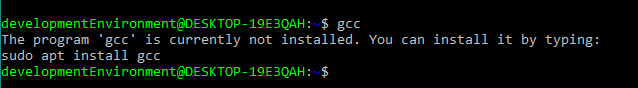
\includegraphics[width=.75\textwidth]{1.png}
\caption{Terminal}
\label{fig:exampleFig1}
\end{figure}

\pagebreak Como sugerido na imagem, inserimos o comando: \textit{sudo apt-get install gcc}. Após realização do download o compilador GCC será instalado automaticamente.

\subsubsection{Utilização}
Com o GCC já instalado no seu sistema, é muito simples usá-lo para compilar programas em C. Se o programa consistir de um único arquivo, você pode simplesmente executar este comando no terminal:

\textit{gcc prog.c -o prog}

onde prog.c é o nome do arquivo que contém o código. É preciso especificar o nome do arquivo executável de saída,pois, o padrão por razões históricas, é usar o arquivo a.out. Em geral, é utilizado o mesmo nome do arquivo de código, tirando a extensão .c. Nesse caso, foi utilizado \textit{prog}.
Para executar o programa, a maneira mais “universal” é digitar o seguinte comando no terminal:

\textit{./prog}

\subsection{GDB - GNU Debugger}

O GDB também conhecido como GNU Debugger, oferece várias facilidades para a depuração de programas. O usuário pode monitorar e alterar valores de variáveis internas do sistema, e até chamar funções de forma independente do fluxo do programa \cite{stallman1988debugging}. Além de ser compatível com várias linguagens de programação.

\subsubsection{Instalação}

Para efetuar a instalação do GDB - GNU Debugger, com o terminal aberto, inserir os seguintes comandos:

\textit{sudo apt-get update} e \textit{sudo apt-get install gdb}.\\\\ 
Sendo que o primeiro irá verificar alguma atualização do sistema, e o segundo para download e instalação do depurador.

\subsubsection{Utilização}

Para realizar a depuração com o GDB, é necessário adicionar a flag -g na hora da compilação com o GCC. Desta maneira, o compilador fica ciente que incluiremos o depurador no executável. Exemplo:

\textbf{No terminal:}
\textit{gcc prog.c -g -o prog}\\\\
Executando o programa com o GDB:\\

\textit{gdb ./prog}

\section{NASM - Netwide Assembler}

Considerado um dos montadores mais populares para o Linux o Netwide Assembler (NASM) é um montador e desmontador para a arquitetura Intel x86 \cite{tatham2011netwide}. Ele pode ser usado para escrever programas de 16 bits, 32 bits (IA-32) e 64 bits (x86-64).

\subsubsection{Instalação}

Para realização da instalação, será efetuada a inserção do comando no terminal semelhante como foi feito anteriormente:

\textit{sudo apt-get install nasm}\\

\subsubsection{Utilização}

\begin{itemize}
\item Criando o Source File
	\subitem Você pode usar qualquer editor de texto, como Gedit, KWrite ou XEmacs, para fazê-lo. Quando você salvar seu arquivo, dê a extensão .asm.
\item Montando o Source File
	\subitem Use a seguinte linha de comando para montar seu arquivo de origem:
    
		\textit{nasm -f elf test.asm}
    
    No exemplo, o arquivo .asm salvo é chamado test.asm. Isso criará um arquivo chamado test.o no diretório atual. Este arquivo não é executável. Ainda é um arquivo de objeto.
\item Criando o executável
	\subitem Agora que temos o nosso arquivo de objeto, chamado test.o, devemos criar nosso arquivo executável.Seu programa pode começar com um procedimento chamado _start. Isso significa que seu programa tem seu próprio ponto de entrada, sem o uso da função principal. No entanto, você precisará usar o "l" para criar seu executável:
    
    	\textit{ld test.o -o test}
    
    Alternativamente, seu programa pode começar com um procedimento chamado main. Você precisará usar gcc para criar seu executável:

		\textit{test.o -o test} 
\item Execução do Programa
	\subitem Para executar o programa chamado test, basta digitar o seguinte comando:
    \textit{./ test}
Agora, seu executável é criado, testado e localizado no diretório atual.
\end{itemize}

\section{ObjDump}

O comando Objdump no Linux é usado para fornecer informações detalhadas sobre arquivos de objeto \cite{santosa2006understanding}. Este comando é usado principalmente pelos programadores que trabalham em compiladores, mas ainda é uma ferramenta muito útil para programadores normais também quando se trata de depuração.Por ser uma ferramenta nativa, não necessita de instalação. Porém, para verificar sua versão instalada, é necessário entrar com o comando:

\textit{objdump --version}

No caso atual, foi exibida a seguinte informação:
\begin{figure}[ht]
\centering
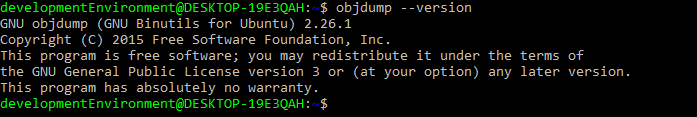
\includegraphics[width=.75\textwidth]{2.png}
\caption{Versão ObjDump}
\label{fig:exampleFig1}
\end{figure}

\subsubsection{Utilizaçao}
São várias as opções de utilização do ObjDump, dentre elas podemos citar a flag -C que é capaz de decodificar (demangle) nomes de símbolos de baixo nível em nomes de nível de usuário. Além de remover qualquer rascunho inicial previamente feito pelo sistema, isso torna os nomes de funções C ++ legíveis. Outras opções podem ser encontradas inserindo a flag -H que mostra na tela o resumo das opções \textit{ObjDump} e sai.

\section{KDbg}

O KDbg é uma interface de usuário gráfica para o depurador GNU. Ele fornece uma interface intuitiva para definir pontos de interrupção, inspecionar variáveis e percorrer o código \cite{sixt2009kdbg}.

\subsubsection{Instalação}

Para realizar a instalação do KDgb, o seguinte procedimento deve ser realizado no terminal:

\begin{figure}[ht]
\centering
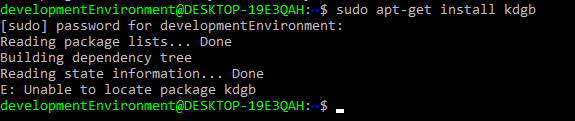
\includegraphics[width=.75\textwidth]{3.png}
\caption{Instalação do KDgb}
\label{fig:exampleFig1}
\end{figure}

\section{Bless Hex Editor}

O Bless é um aplicativo de editor hexadecimal de código aberto usado para criar e editar arquivos hexadecimais.

\subsubsection{Instalação}
Para realizar a instalação atualize seu sistema com o comando:

\textit{sudo apt-get update}

Logo em seguida, insira o comando:

\textit{sudo apt-get install bless}

Talvez seja necessário inserir a senha de usuário cadastrada. No entanto, após a inserção da senha, o terminal se encarregará de fazer o download e realizar a instalação.
Para verificar se a instalação foi realizada com sucesso, insira o seguite comando:

\textit{sudo dpkg -l bless}

Será exibida a seguinte mensagem:

\begin{figure}[ht]
\centering
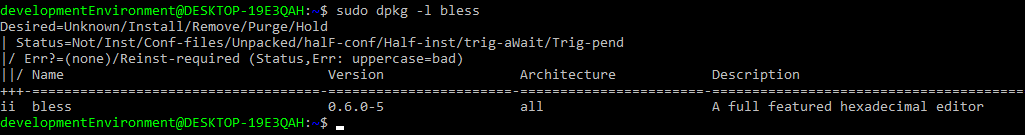
\includegraphics[width=.75\textwidth]{4.png}
\caption{Verificação da versão do Editor Bless}
\label{fig:exampleFig1}
\end{figure}

\section{Editor de texto}

Será utilizado o editor de texto Sublime Text 3, já instalada e disponível na máquina Windows.

\bibliographystyle{sbc}
\bibliography{sbc-template}

\end{document}
